\chapter{10要素の動作検証}\label{chap:4}

\section{入力コピーと開始同期}\label{sec:4-1}

指定入力は7, 1, 4, 9, 3, 8, 2, 6, 5, 0である。
Core0は前半5要素、Core1は後半5要素を担当する。
図\ref{fig:2}に処理順を示す。
READYが立つまでCore1を待たせ、入力コピーの途中でソートが始まらないようにする。



\begin{figure}[H]

\centering

\begin{tikzpicture}[x=\dimexpr\linewidth/500\relax,y=-1pt,>=stealth]
\draw[->,line width=0.5pt] (99,70) -- (99,90);
\draw[->,line width=0.5pt] (400,70) -- (400,90);
\draw[->,line width=0.5pt] (99,126) -- (99,146);
\draw[->,line width=0.5pt] (400,126) -- (400,146);
\draw[->,line width=0.5pt] (99,187) -- (99,207);
\draw[->,line width=0.5pt] (400,187) -- (400,207);
\draw[->,line width=0.5pt] (99,248) -- (99,268);
\draw[->,line width=0.5pt] (400,248) -- (400,268);
\draw[->,line width=0.5pt] (198,48) -- (301,48);
\draw[->,line width=0.5pt] (301,168) -- (198,168);
\draw[->,line width=0.5pt] (198,290) -- (301,290);
\node[align=center,inner sep=2pt,text width=0.38000\linewidth,minimum height=48pt,draw=black!50,fill=black!3] at (99.0,46.0) {\fontsize{9}{11.700000000000001}\selectfont フラグを0に初期化\\入力をROMからRAMへコピー\\READYを1にする};
\node[align=center,inner sep=2pt,text width=0.38000\linewidth,minimum height=48pt,draw=black!50,fill=black!3] at (400.0,46.0) {\fontsize{9}{11.700000000000001}\selectfont READYが1になるまで待機\\入力の準備ができたら進む};
\node[align=center,inner sep=2pt,text width=0.38000\linewidth,minimum height=36pt,draw=black!50,fill=black!3] at (99.0,108.0) {\fontsize{9}{11.700000000000001}\selectfont 前半をバブルソート\\floor(N/2)要素};
\node[align=center,inner sep=2pt,text width=0.38000\linewidth,minimum height=36pt,draw=black!50,fill=black!3] at (400.0,108.0) {\fontsize{9}{11.700000000000001}\selectfont 後半をバブルソート\\残りの要素};
\node[align=center,inner sep=2pt,text width=0.38000\linewidth,minimum height=41pt,draw=black!50,fill=black!3] at (99.0,166.5) {\fontsize{9}{11.700000000000001}\selectfont LEFT\_DONEを1にする\\RIGHT\_DONEが1になるまで待機};
\node[align=center,inner sep=2pt,text width=0.38000\linewidth,minimum height=41pt,draw=black!50,fill=black!3] at (400.0,166.5) {\fontsize{9}{11.700000000000001}\selectfont RIGHT\_DONEを1にする};
\node[align=center,inner sep=2pt,text width=0.38000\linewidth,minimum height=41pt,draw=black!50,fill=black!3] at (99.0,227.5) {\fontsize{9}{11.700000000000001}\selectfont 二つの区間を作業領域へマージ\\配列領域へ結果を書き戻す};
\node[align=center,inner sep=2pt,text width=0.38000\linewidth,minimum height=41pt,draw=black!50,fill=black!3] at (400.0,227.5) {\fontsize{9}{11.700000000000001}\selectfont COMPLETEが1になるまで待機};
\node[align=center,inner sep=2pt,text width=0.38000\linewidth,minimum height=41pt,draw=black!50,fill=black!3] at (99.0,288.5) {\fontsize{9}{11.700000000000001}\selectfont COMPLETEを1にする\\終端ループへ移る};
\node[align=center,inner sep=2pt,text width=0.38000\linewidth,minimum height=41pt,draw=black!50,fill=black!3] at (400.0,288.5) {\fontsize{9}{11.700000000000001}\selectfont COMPLETEを確認\\終端ループへ移る};
\node[align=center,inner sep=2pt,text width=0.38000\linewidth,minimum height=20pt] at (99.0,10.0) {\fontsize{10}{13.0}\selectfont \bfseries Core0};
\node[align=center,inner sep=2pt,text width=0.38000\linewidth,minimum height=20pt] at (400.0,10.0) {\fontsize{10}{13.0}\selectfont \bfseries Core1};
\node[align=center,inner sep=2pt,text width=0.16000\linewidth,minimum height=17pt] at (249.0,36.5) {\fontsize{9}{11.700000000000001}\selectfont READY};
\node[align=center,inner sep=2pt,text width=0.16000\linewidth,minimum height=17pt] at (249.0,156.5) {\fontsize{9}{11.700000000000001}\selectfont RIGHT\_DONE};
\node[align=center,inner sep=2pt,text width=0.16000\linewidth,minimum height=17pt] at (249.0,278.5) {\fontsize{9}{11.700000000000001}\selectfont COMPLETE};
\end{tikzpicture}


\caption{開始通知、担当区間のソート、完了通知、マージの順序。フラグの1への更新は処理の担当コアが行う。}\label{fig:2}

\end{figure}

\par\medskip\noindent\begin{minipage}{\linewidth}
\par\medskip\noindent{\small\bfseries コード3　ROMからのコピーと前半ソート　listing.s}\par\nopagebreak

\lstinputlisting{code/code-03.txt}
\end{minipage}\par\medskip

コード3の2048は0x0800、4352は0x1100である。
Core0はROMからRAMへ10要素をコピーしてから、17行目でREADYに1を書く。
次にCore0はソート処理を呼び出し、前半5要素を整列させる。
フラグの初期クリアとCore1側の入口は付録Aの8〜11行、31〜43行に示す。



\section{ソート完了の同期}\label{sec:4-2}

\par\medskip\noindent\begin{minipage}{\linewidth}
\par\medskip\noindent{\small\bfseries コード4　左側完了の通知と右側完了の待機　listing.s}\par\nopagebreak

\lstinputlisting{code/code-04.txt}
\end{minipage}\par\medskip

Core0はLEFT\_DONEへ1を書いた後、RIGHT\_DONEを繰り返し読む。
Core1は自分のソートが終わるとRIGHT\_DONEへ1を書き、その後はCOMPLETEを待つ。
固定時間の遅延ではなく、各処理の完了を次の処理の開始条件にしている。



\begin{figure}[H]

\centering

\noindent\makebox[\linewidth][l]{\small (a) 開始〜約1,900 ns}\par\smallskip

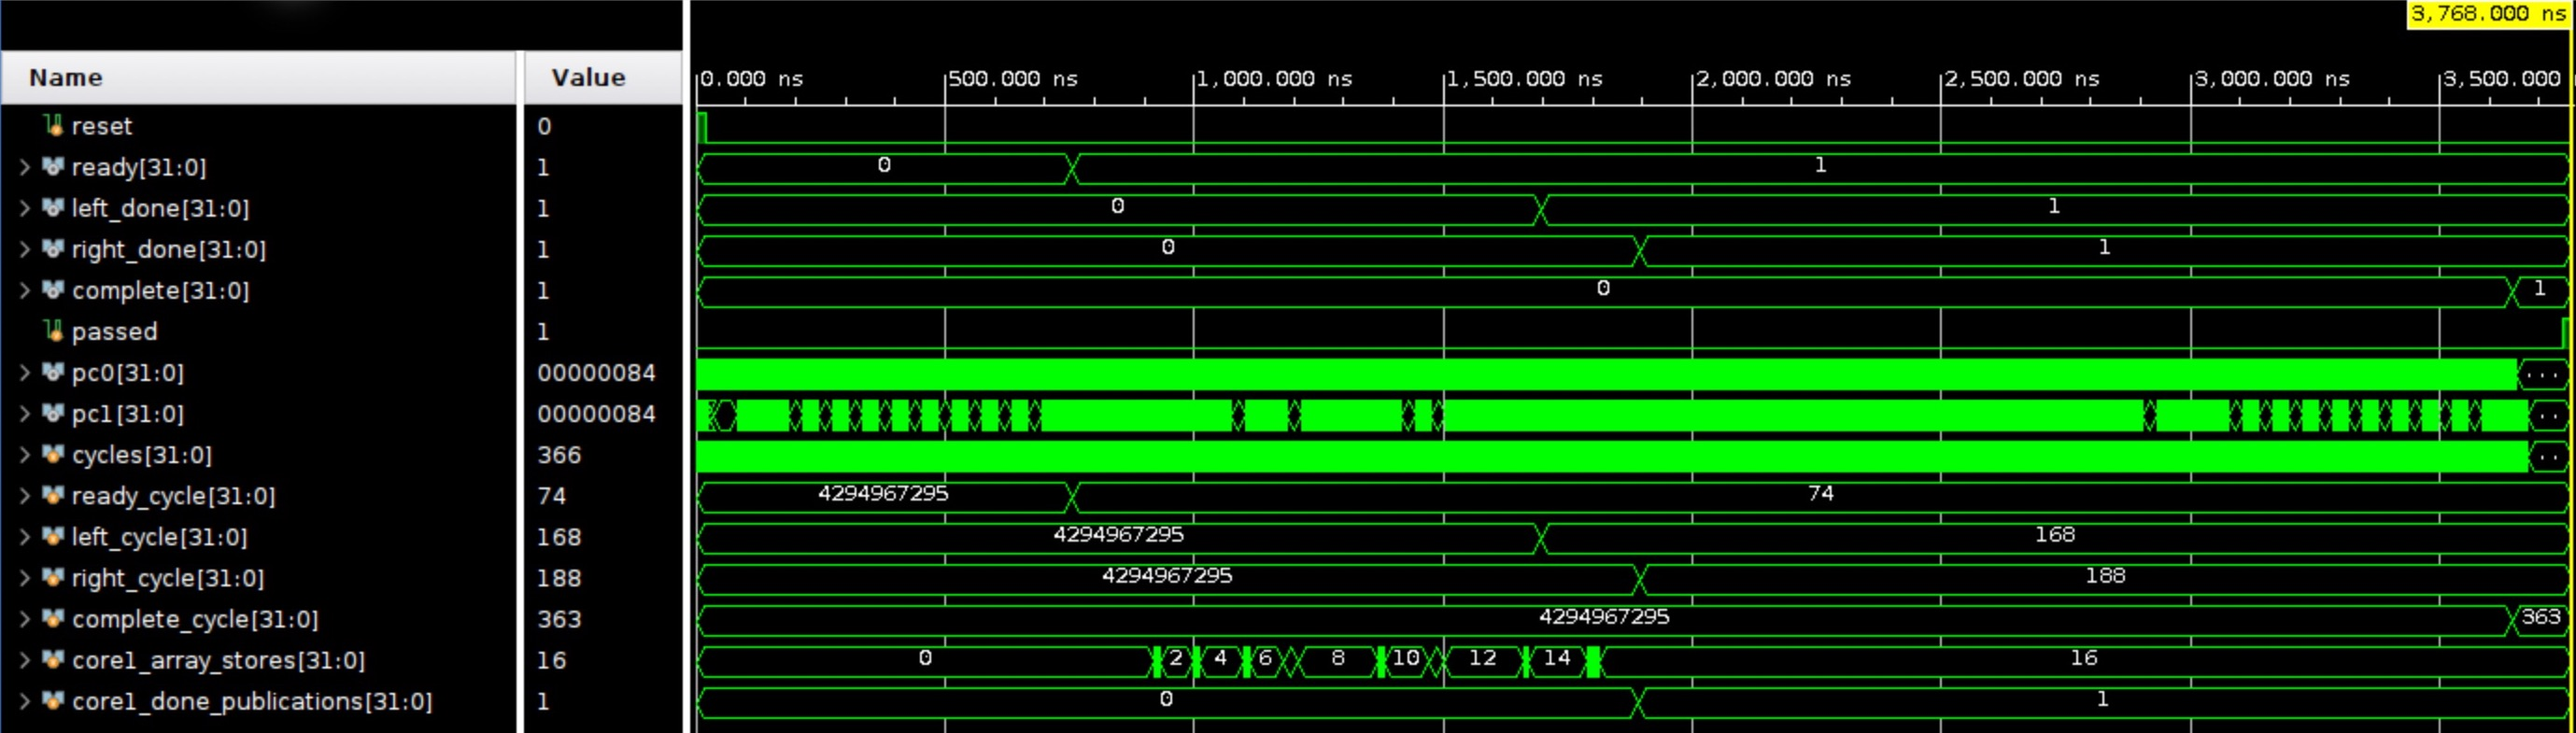
\includegraphics[bb=0 0 2758 785,viewport=0 403 410 785,clip,width=.261\linewidth]{figures/02-synchronization-wave.png}%
\hspace{.005\linewidth}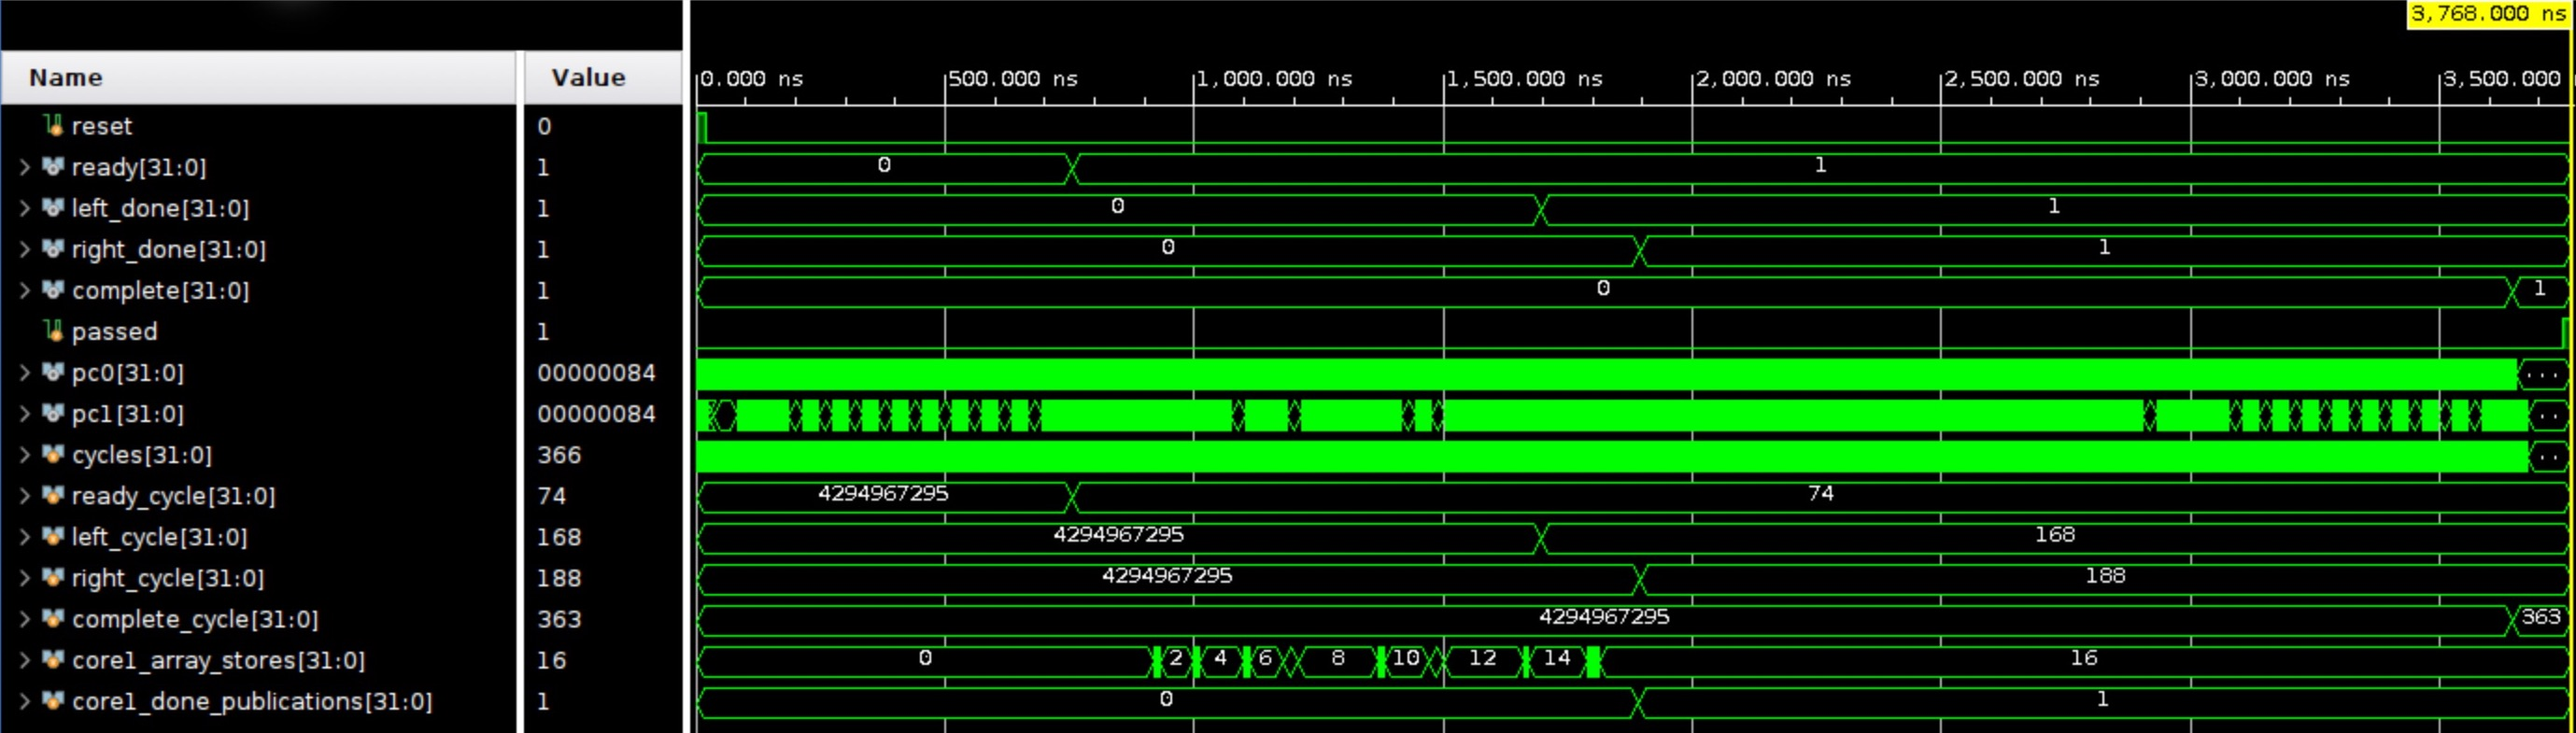
\includegraphics[bb=0 0 2758 785,viewport=555 403 675 785,clip,width=.076\linewidth]{figures/02-synchronization-wave.png}%
\hspace{.005\linewidth}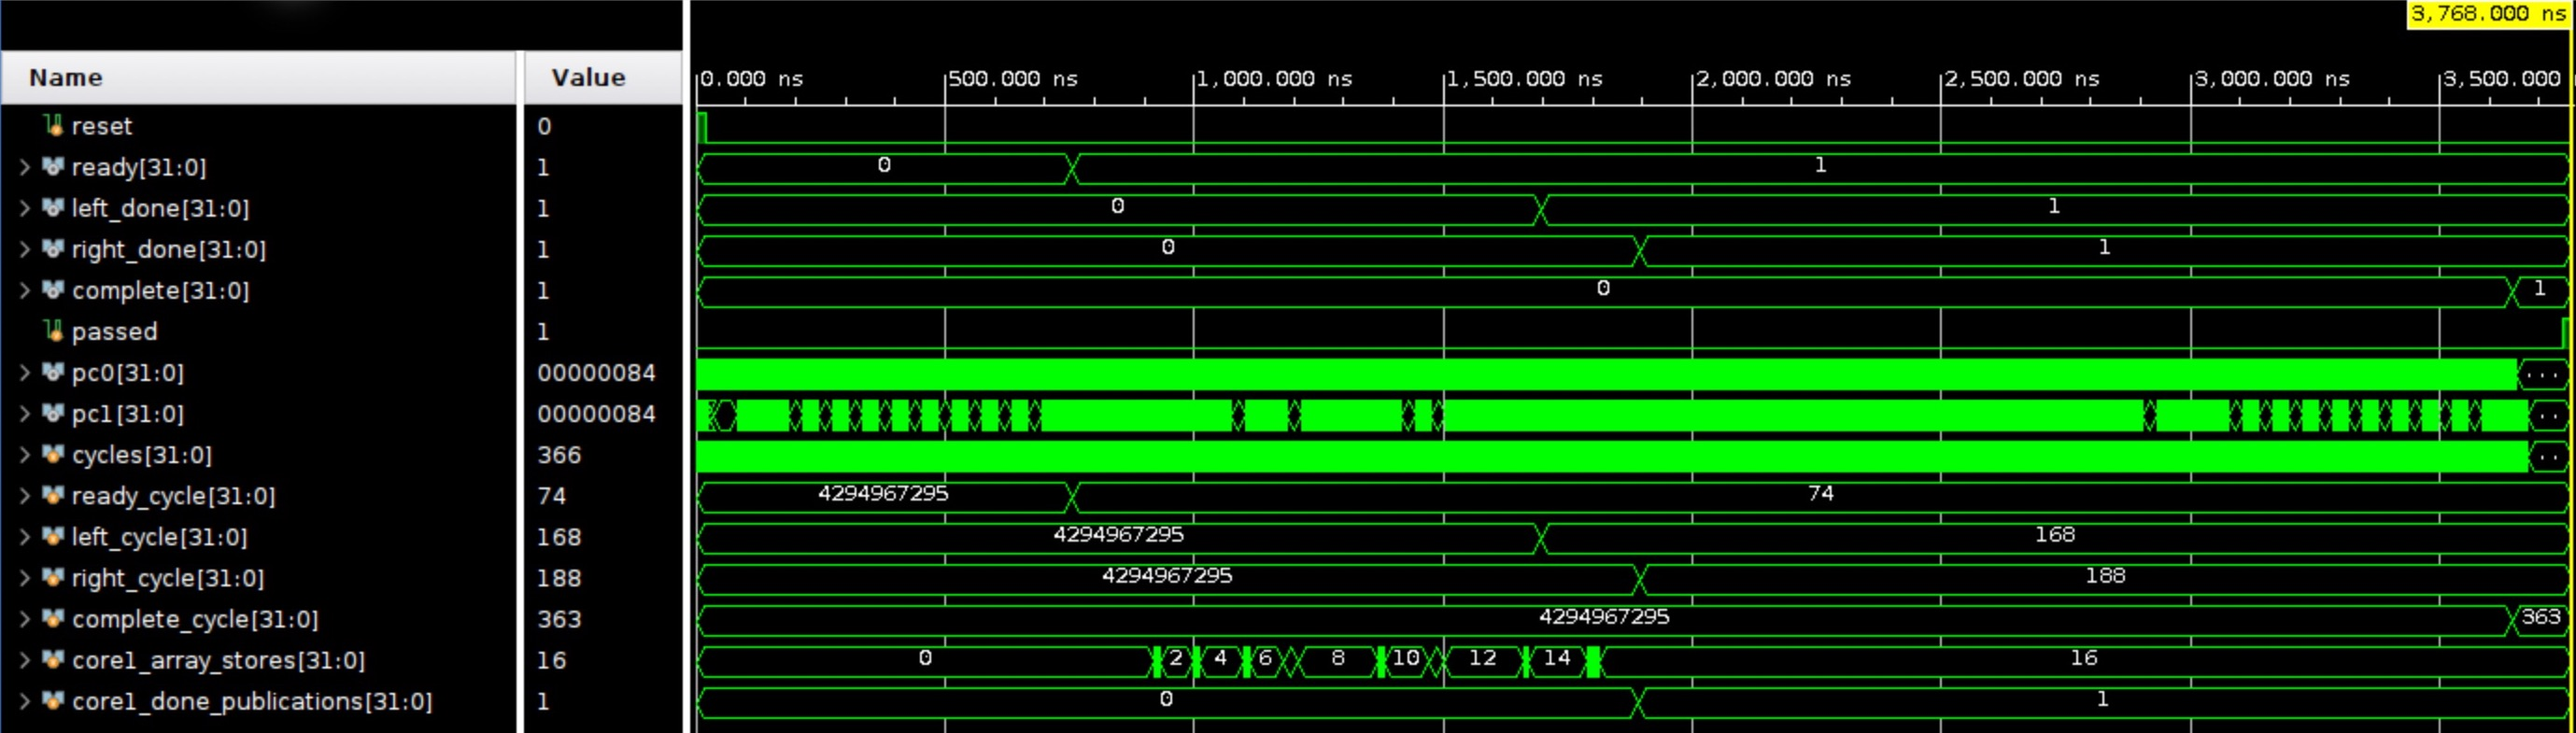
\includegraphics[bb=0 0 2758 785,viewport=742 403 1750 785,clip,width=.643\linewidth]{figures/02-synchronization-wave.png}\par\medskip

\noindent\makebox[\linewidth][l]{\small (b) 約1,900 ns〜終了}\par\smallskip

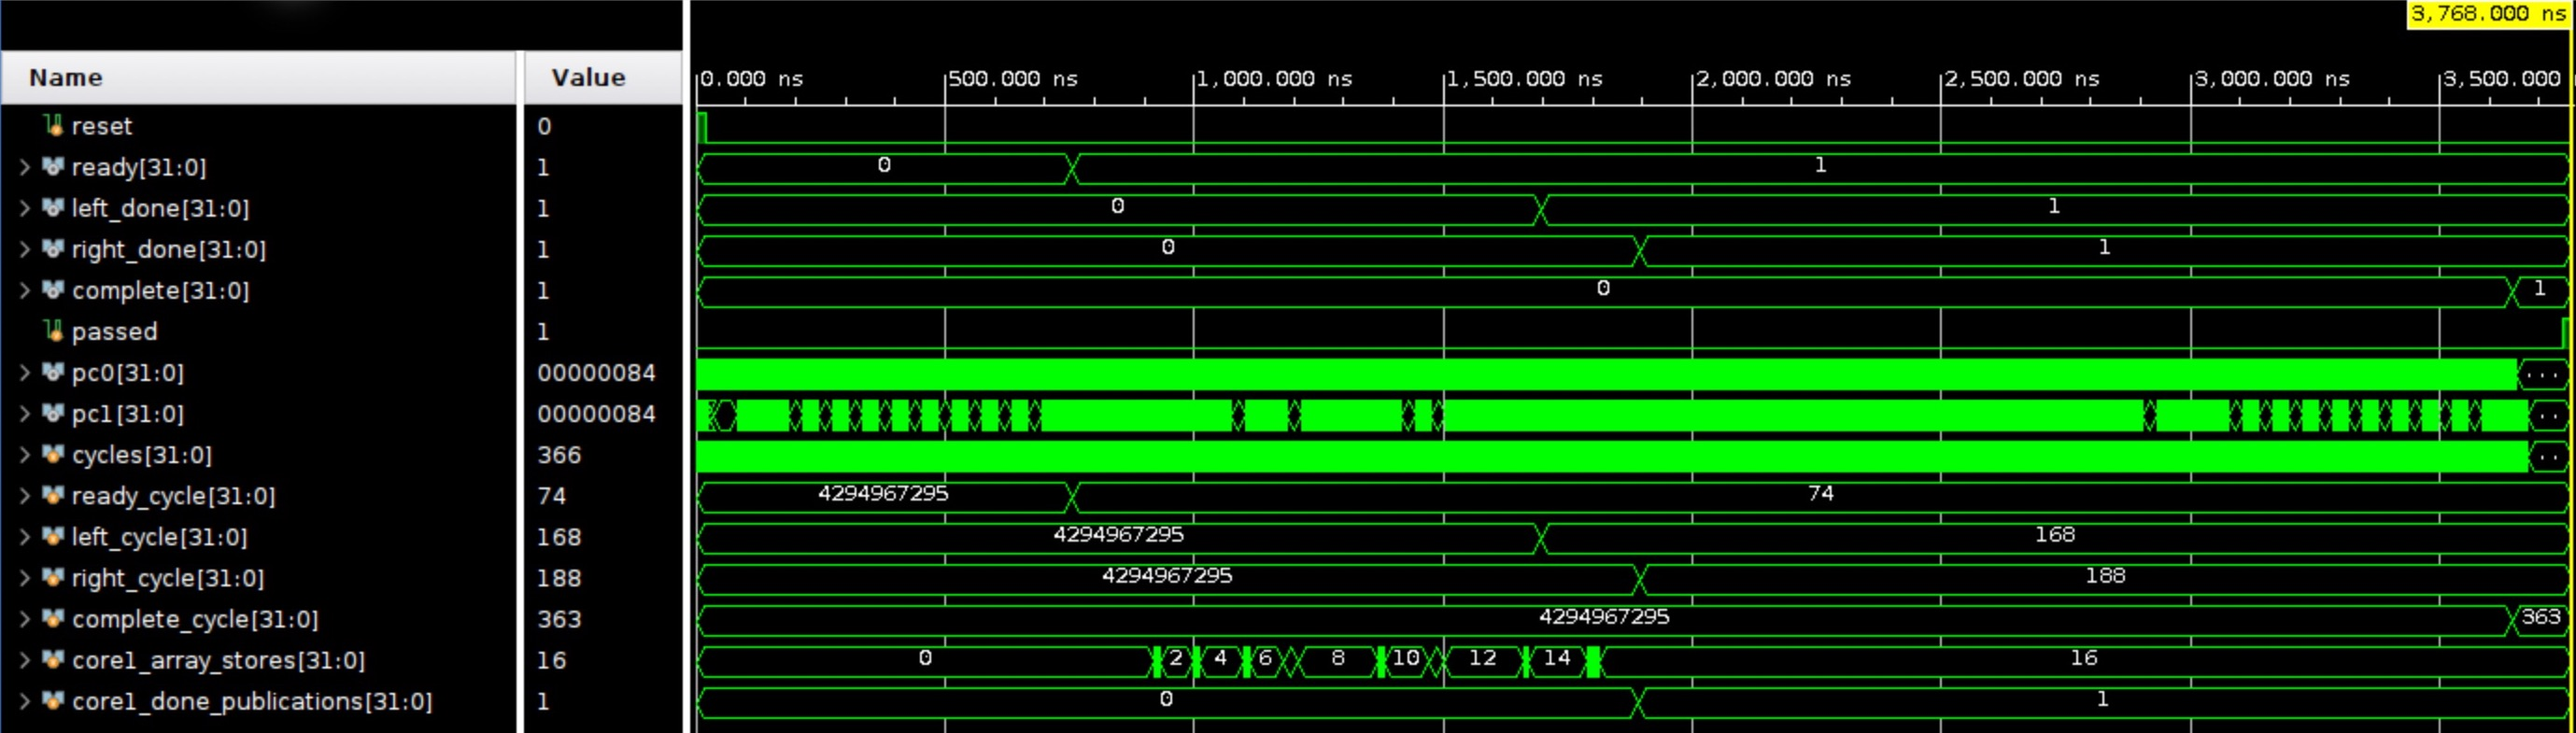
\includegraphics[bb=0 0 2758 785,viewport=0 403 410 785,clip,width=.261\linewidth]{figures/02-synchronization-wave.png}%
\hspace{.005\linewidth}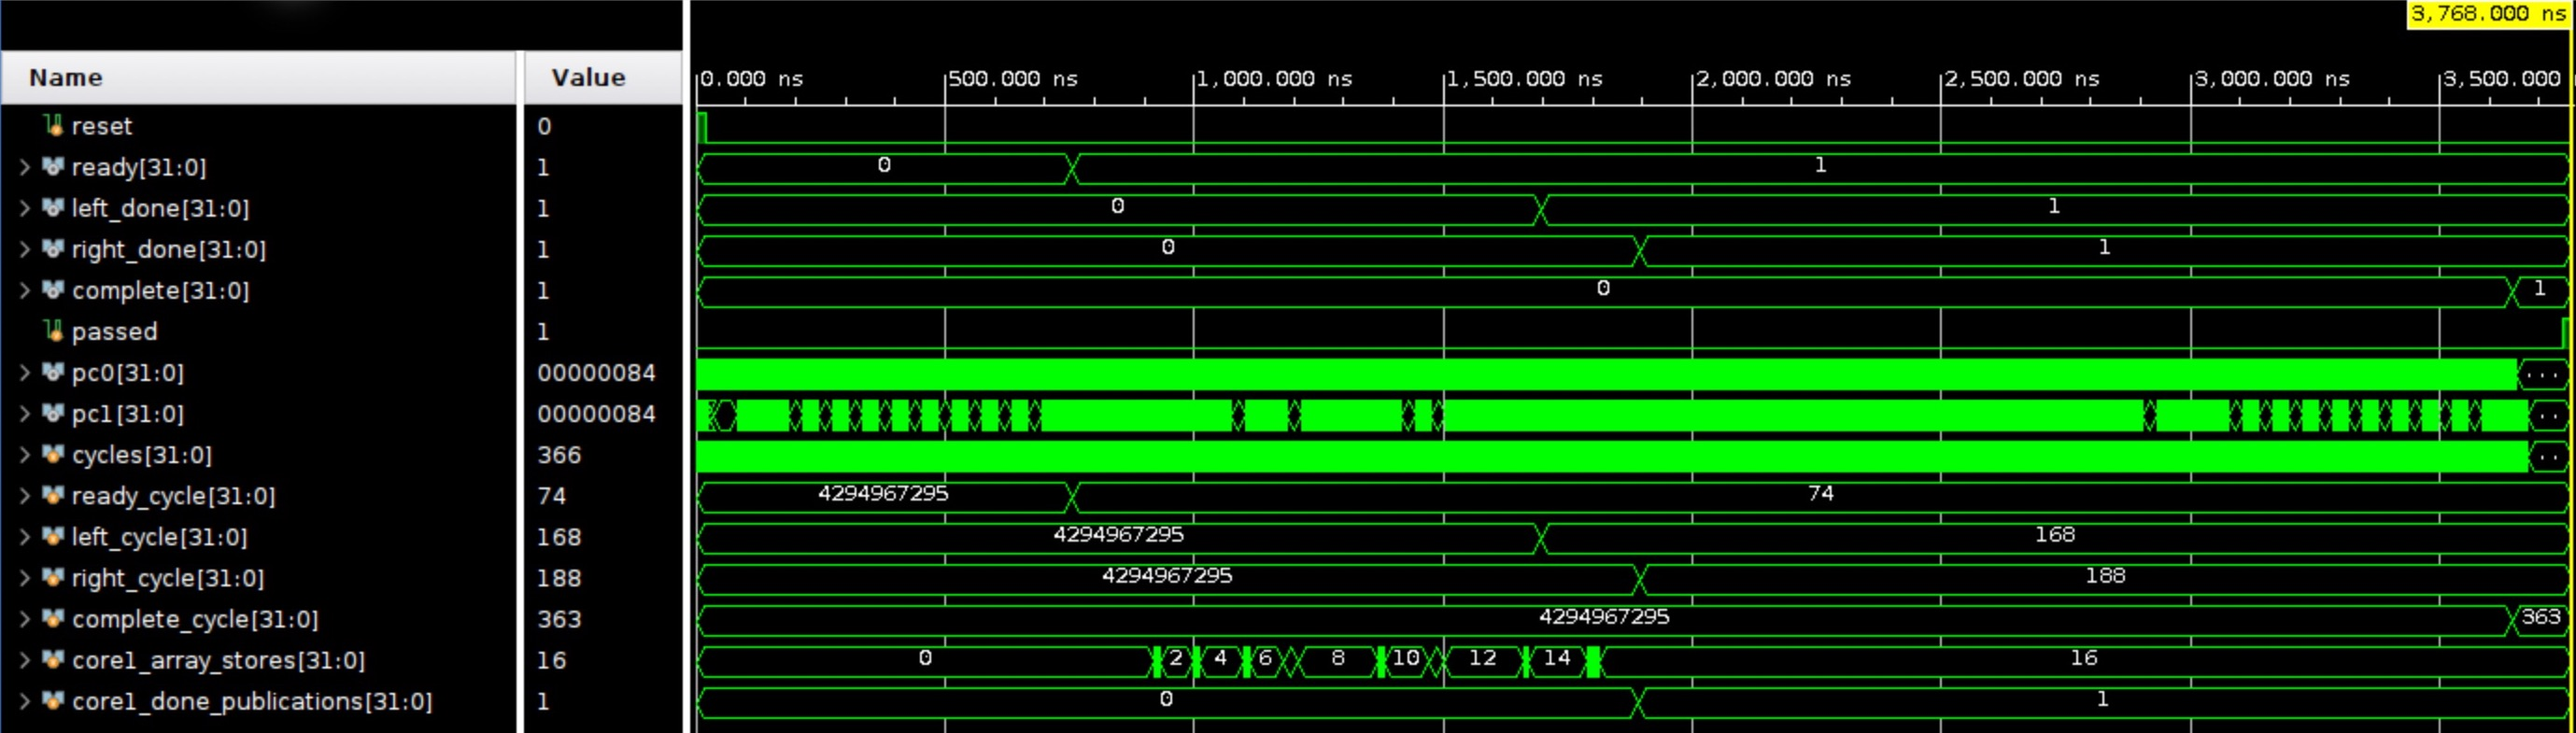
\includegraphics[bb=0 0 2758 785,viewport=555 403 675 785,clip,width=.076\linewidth]{figures/02-synchronization-wave.png}%
\hspace{.005\linewidth}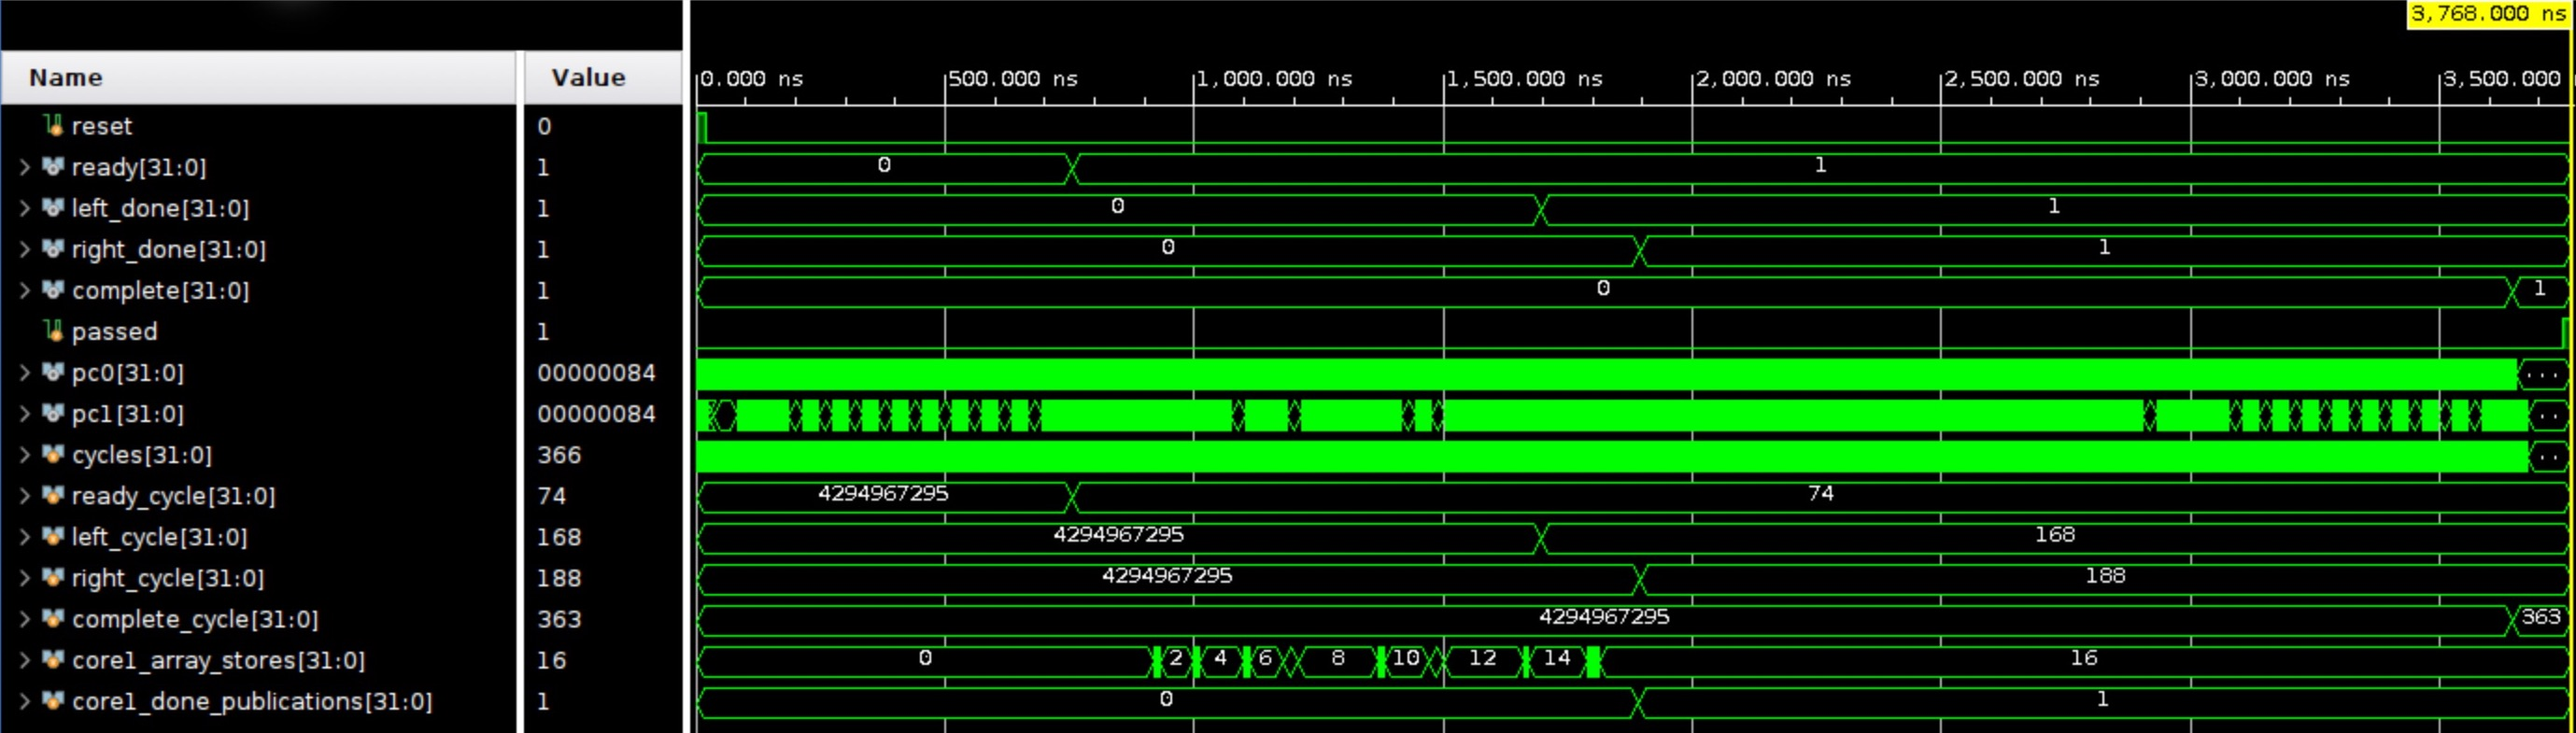
\includegraphics[bb=0 0 2758 785,viewport=1750 403 2758 785,clip,width=.643\linewidth]{figures/02-synchronization-wave.png}\par\medskip

\caption{10要素dual実行の完了フラグ。上下は同じ実行の前半と後半で、信号名を繰り返した。Value列は最終カーソル時点の値。横軸nsとリセット解除基準のcyclesは原点が異なる。}\label{fig:3}

\end{figure}

\begin{table}[H]

\centering

\caption{図3に対応する初回観測サイクル}

\label{tab:4}

\footnotesize

\setlength{\tabcolsep}{3pt}

\renewcommand{\arraystretch}{1.25}

\begin{tabular}{>{\raggedright\arraybackslash}p{\dimexpr0.180261\linewidth-2\tabcolsep\relax}>{\raggedright\arraybackslash}p{\dimexpr0.208302\linewidth-2\tabcolsep\relax}>{\raggedright\arraybackslash}p{\dimexpr0.208302\linewidth-2\tabcolsep\relax}>{\raggedright\arraybackslash}p{\dimexpr0.202293\linewidth-2\tabcolsep\relax}>{\raggedright\arraybackslash}p{\dimexpr0.200842\linewidth-2\tabcolsep\relax}}\toprule

\textbf{READY} & \textbf{LEFT\_DONE} & \textbf{RIGHT\_DONE} & \textbf{COMPLETE} & \textbf{参加コア終端}\\\midrule

74 & 168 & 188 & 363 & 366\\

\bottomrule\end{tabular}

\end{table}

波形では、左側の完了が168サイクル目、右側の完了が188サイクル目に観測された（図\ref{fig:3}、表\ref{tab:4}）。
Core0は右側の完了を確認してからマージと書き戻しを行い、363サイクル目にCOMPLETEを立てた。Core1がこれを確認し、参加コアが終端に達するまでを数えると366サイクルだった。



Core1による配列への書込みは16回受理され、右側の完了通知もCore1が1回書き込んだ。書込み先が担当区間内であることと、通知元がCore1であることはテストベンチで照合した（付録C）。



\section{競合時の状態保持と実行再開}\label{sec:4-3}

\par\medskip\noindent\begin{minipage}{\linewidth}
\par\medskip\noindent{\small\bfseries コード5a　Core0優先の調停とストール　simple\_memory\_arbiter.v}\par\nopagebreak

\lstinputlisting{code/code-05.txt}
\end{minipage}\par\medskip

req0とreq1が同時に1になると、Core0が許可され、Core1のstall1が1になる。
CPU側ではRegWriteを!stallで抑止し、PCも!stallのときだけ更新する。
この機構は既存のCPUから引き継いだ。



\par\medskip\noindent\begin{minipage}{\linewidth}
\par\medskip\noindent{\small\bfseries コード5b　レジスタ書込みとPC更新の抑止　simple\_cpu\_with\_mem\_interface.v}\par\nopagebreak

\lstinputlisting{code/code-06.txt}
\end{minipage}\par\medskip

\par\medskip\noindent\begin{minipage}{\linewidth}
\par\medskip\noindent{\small\bfseries コード6　隣接要素の比較と交換　listing.s}\par\nopagebreak

\lstinputlisting{code/code-07.txt}
\end{minipage}\par\medskip

このCPUのsltは符号なし比較である。
後ろの要素の値が小さければ、74〜75行で二つの要素を交換する。



\begin{figure}[H]

\centering

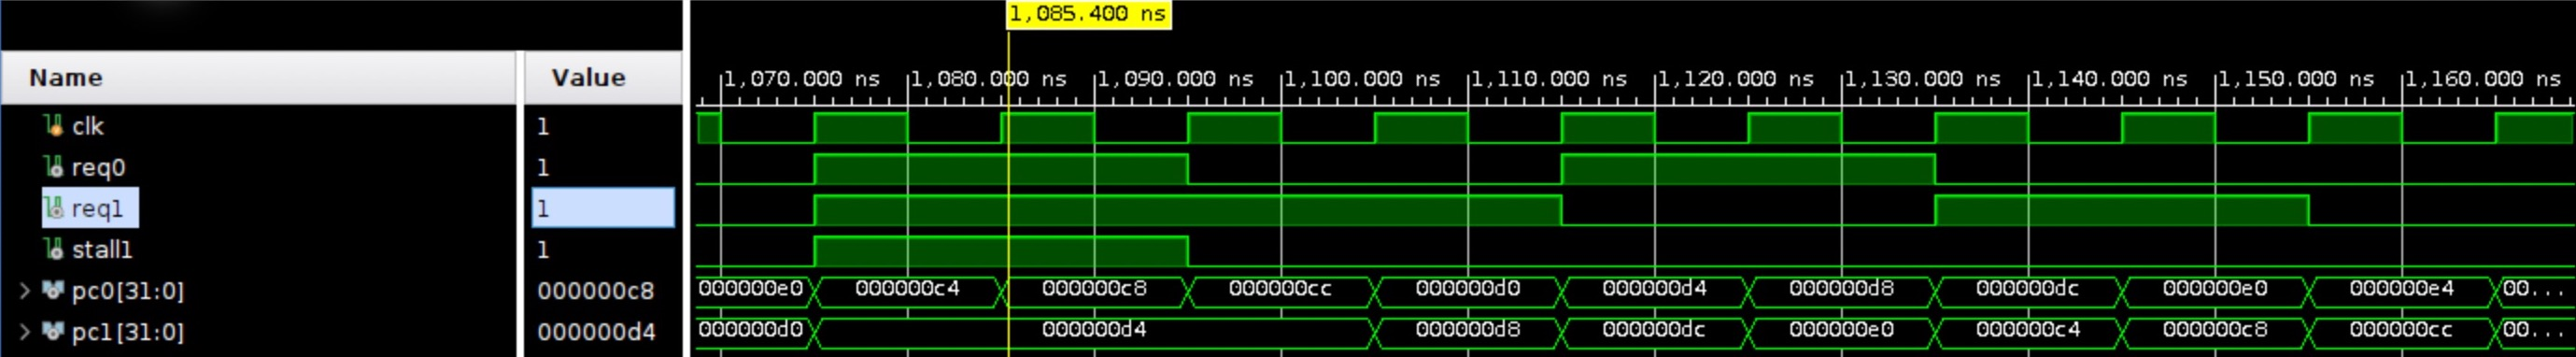
\includegraphics[bb=0 0 2758 382,viewport=0 0 1950 382,clip,width=\linewidth]{figures/03-contention-wave.png}

\caption{1085.4 ns付近の同時要求。req0、req1、stall1が1で、PC0は0xC8、PC1は0xD4を示す。Core1のPCは競合区間をまたいで保持され、待機解除後に0xD8へ進む。}\label{fig:4}

\end{figure}

付録AのPC注記と照合すると、0xC8はコード6の71行目のload、0xD4は74行目の最初のstoreである。
図\ref{fig:4}ではCore1のPCが1075〜1095 nsの競合区間をまたいで0xD4に留まる。
再開後の0xD8は75行目の次のstoreに対応する。



この実行でCore1がストールしたのは計77サイクルだった。図\ref{fig:4}ではその一例としてPCの保持と再開を示す。
テストベンチでは、ストールしたクロック端の前後でPCと全32レジスタを照合した（付録C.2）。



\section{マージ処理と最終配列の確認}\label{sec:4-4}

両側の完了後、Core0は整列済み区間の先頭を比較し、小さい値を0x1300からの作業領域へ書く。
同値では左側を選ぶ。
一方の区間を使い切ったら残りを転送し、作業領域の10要素を0x1100へ書き戻す。
付録Aに分岐と残り要素の処理を含む一覧を示す。



\par\medskip\noindent\begin{minipage}{\linewidth}
\par\medskip\noindent{\small\bfseries コード7　マージの比較と最後の書き戻し　listing.s}\par\nopagebreak

\lstinputlisting{code/code-08.txt}
\end{minipage}\par\medskip

\begin{figure}[H]

\centering

\begin{minipage}{.43\linewidth}

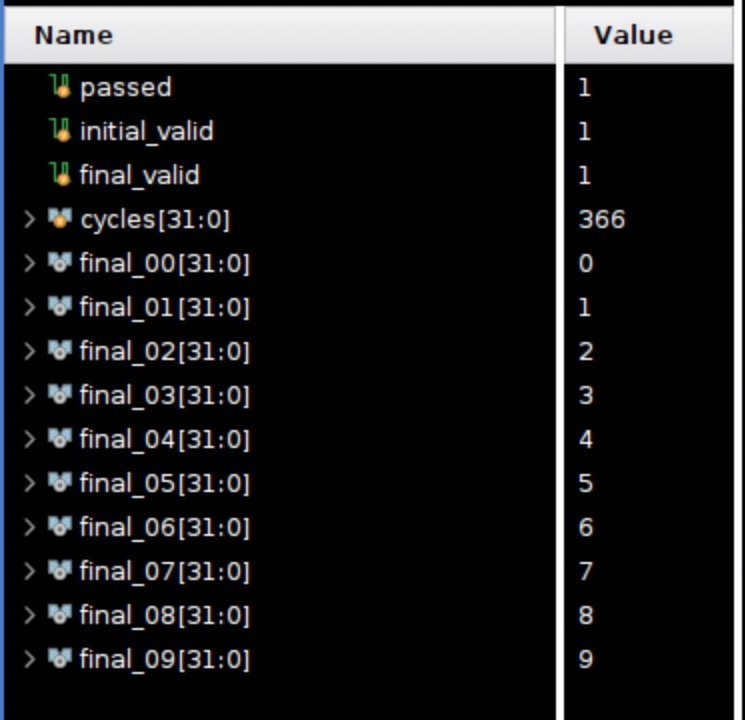
\includegraphics[width=\linewidth]{figures/01a-correctness-values.png}

\end{minipage}\hfill\begin{minipage}{.51\linewidth}

\small 入力\par 7,1,4,9,3,8,2,6,5,0\par \par 出力\par 0,1,2,3,4,5,6,7,8,9\par \par Core1の受理された配列storeは16回。自分の完了通知は1回だった。

\end{minipage}

\caption{最終スナップショット。final\_00〜final\_09は0〜9、cyclesは366。initial\_validは入力コピーの照合、final\_validは最終値の取得、passedは検査通過を示す。}\label{fig:5}

\end{figure}

\par\medskip\noindent\begin{minipage}{\linewidth}
\par\medskip\noindent{\small\bfseries コード8　保存した最終値と検査通過の公開　tb\_vivado\_sort.v}\par\nopagebreak

\lstinputlisting{code/code-09.txt}
\end{minipage}\par\medskip

図\ref{fig:5}は同じten-dual-v2実行の波形で、マージ後の配列が0から9まで昇順に並んでいる。
final\_validは最終値を取り込んだこと、passedは期待値との照合を含む検査を通過したことを示す。
この波形に表示したのはマージ後の配列で、左右それぞれのソート直後の配列ではない。


